\chapter*{Proposition 46}



\begin{figure*}[ht]
    \begin{center}
    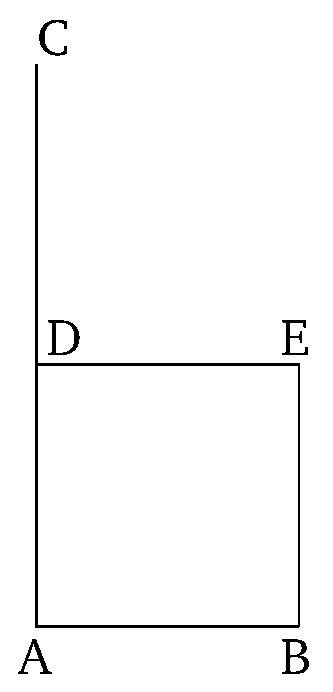
\includegraphics[width=0.5\linewidth]{figures/fig46e.eps}
    \label{fig:prop_46}
    \end{center}
\end{figure*}

To describe a square on a given straight-line.

Let $AB$ be the given straight-line. So it is required to describe a
square on the straight-line $AB$.

Let $AC$ have been drawn at right-angles to the straight-line $AB$
from the point $A$ on it [Prop.~1.11], and let $AD$ have been
made equal to $AB$ [Prop.~1.3]. And let $DE$ have been drawn
through point $D$ parallel to $AB$ [Prop.~1.31], and let $BE$ have been
drawn through point $B$ parallel to $AD$ [Prop.~1.31]. Thus,
$ADEB$ is a parallelogram. Therefore, $AB$ is equal to $DE$, and $AD$ to $BE$ [Prop.~1.34]. But, $AB$ is equal to $AD$. Thus, the four (sides) $BA$, $AD$, $DE$, and $EB$ are equal to one another. Thus, the parallelogram $ADEB$ is equilateral.
So I say that (it is) also right-angled. For since the straight-line $AD$ falls
across the parallels $AB$ and $DE$, the (sum of the) angles $BAD$ and $ADE$ is
equal to two right-angles [Prop.~1.29]. But $BAD$ (is a) right-angle. Thus,
$ADE$ (is) also a right-angle. And for parallelogrammic figures, the opposite
sides and angles are equal to one another [Prop.~1.34]. Thus, each of the
opposite angles $ABE$ and $BED$ (are) also right-angles. Thus, $ADEB$ is
right-angled. And it was also shown (to be) equilateral.

Thus, ($ADEB$) is a square [Def.~\ref{def:22}]. And it is described on the straight-line $AB$. (Which is) the very thing it was required to do.


\section*{Commentary}

\begin{proposition}\label{proposition_46}\lean{Elements.Book1.proposition_46}\leanok
    If
\end{proposition}
\begin{proof}
    \uses{proposition_3,proposition_11,proposition_29,proposition_31,proposition_34}\leanok
\end{proof}
